% MORPH — Deployable Stack (precision x training update overlay)
% The deployment-oriented precision scopes plus the training update loop that
% produces those quantized forward weights.
% Compile: pdflatex morph_deploy_stack.tex
%
% NOTE: this diagram tracks base.yaml's deploy-oriented defaults: ternary selected
% backbone weights, int6 Euclidean/bigram embeddings, bf16 attention projections /
% normalization / carriers, and 8-bit AdEMAMix (ademamix_b1zero) optimizer state.

\documentclass[border=16pt]{standalone}
\usepackage[T1]{fontenc}
\usepackage{amsmath,amssymb}
\usepackage{tikz}
\usetikzlibrary{arrows.meta, fit, positioning, calc, backgrounds, decorations.pathreplacing}

% ── Colorblind-safe palette (Paul Tol) ───────────────────────────────────────
\definecolor{cbBlue}{HTML}{4477AA}
\definecolor{cbOrange}{HTML}{EE7733}
\definecolor{cbPurple}{HTML}{AA3377}
\definecolor{cbTeal}{HTML}{228833}
\definecolor{cbGray}{HTML}{777777}

\definecolor{fBlue}{HTML}{DCEAF7}
\definecolor{fOrange}{HTML}{FDE8D0}
\definecolor{fPurple}{HTML}{EEDCEE}
\definecolor{fTeal}{HTML}{D4EDDA}
\definecolor{fGray}{HTML}{EBEBEB}
\definecolor{fYellow}{HTML}{FFF3CD}
\definecolor{bdr}{HTML}{555555}
\definecolor{loopC}{HTML}{2255AA}

% ── Precision palette (colorblind-safe; text label is authoritative, color secondary) ──
\definecolor{pBf16}{HTML}{08519C}   % deep blue
\definecolor{pTern}{HTML}{D55E00}   % vermillion (orange-red)
\definecolor{pInt6}{HTML}{009E73}   % bluish green
\definecolor{pInt4}{HTML}{984EA3}   % purple (distinct from the rest)
\definecolor{p8bit}{HTML}{444444}   % dark gray
\definecolor{pTrain}{HTML}{7A3E9D}  % optimizer / BPTT path
\definecolor{pGrad}{HTML}{CC79A7}   % gradient rail accent

\tikzset{
  % central forward-flow boxes — shared width so braces clear every tier
  L/.style={draw=bdr, thick, rounded corners=4pt,
    minimum width=6.0cm, minimum height=1.0cm,
    font=\small\sffamily, align=center, inner sep=6pt},
  Ls/.style={L, minimum height=0.6cm, font=\footnotesize\sffamily},
  % precision-colored boxes (the box IS the precision label; matches the bottom legend)
  PB/.style={L, draw=pBf16, line width=1pt, fill=pBf16!12},   % bf16  (deep blue)
  PT/.style={L, draw=pTern, line width=1pt, fill=pTern!13},   % ternary (vermillion)
  PI6/.style={L, draw=pInt6, line width=1pt, fill=pInt6!15},  % int6  (green)
  PBs/.style={Ls, draw=pBf16, line width=1pt, fill=pBf16!12}, % bf16 thin (mixer/norm)
  % precision badge (precision ALWAYS spelled out as text — not color-only)
  badge/.style={draw=#1, line width=1pt, rounded corners=3pt,
    fill=#1!18, font=\scriptsize\sffamily\bfseries, text=#1!60!black,
    inner sep=3pt, align=center, minimum height=0.55cm},
  % side callout panels
  panel/.style={draw=#1, very thick, rounded corners=8pt, fill=#1!6,
    inner sep=11pt, align=left, font=\footnotesize\sffamily},
  A/.style={-{Stealth[length=2.6mm,width=2mm]}, thick},
  Ad/.style={-{Stealth[length=2.4mm,width=1.9mm]}, thick, densely dashed},
  TrainA/.style={-{Stealth[length=2.8mm,width=2.2mm]}, line width=1.4pt, densely dashed, draw=pTrain},
  station/.style={draw=#1, thick, rounded corners=5pt, fill=#1!7,
    inner sep=7pt, align=left, font=\scriptsize\sffamily},
  sub/.style={font=\scriptsize\sffamily},
  tiny/.style={font=\tiny\sffamily},
}

% precision-badge helper:  \precb{anchor node}{color}{TEXT}
\newcommand{\precb}[3]{%
  \node[badge=#2, right=0.55cm of #1] {#3};}

\begin{document}
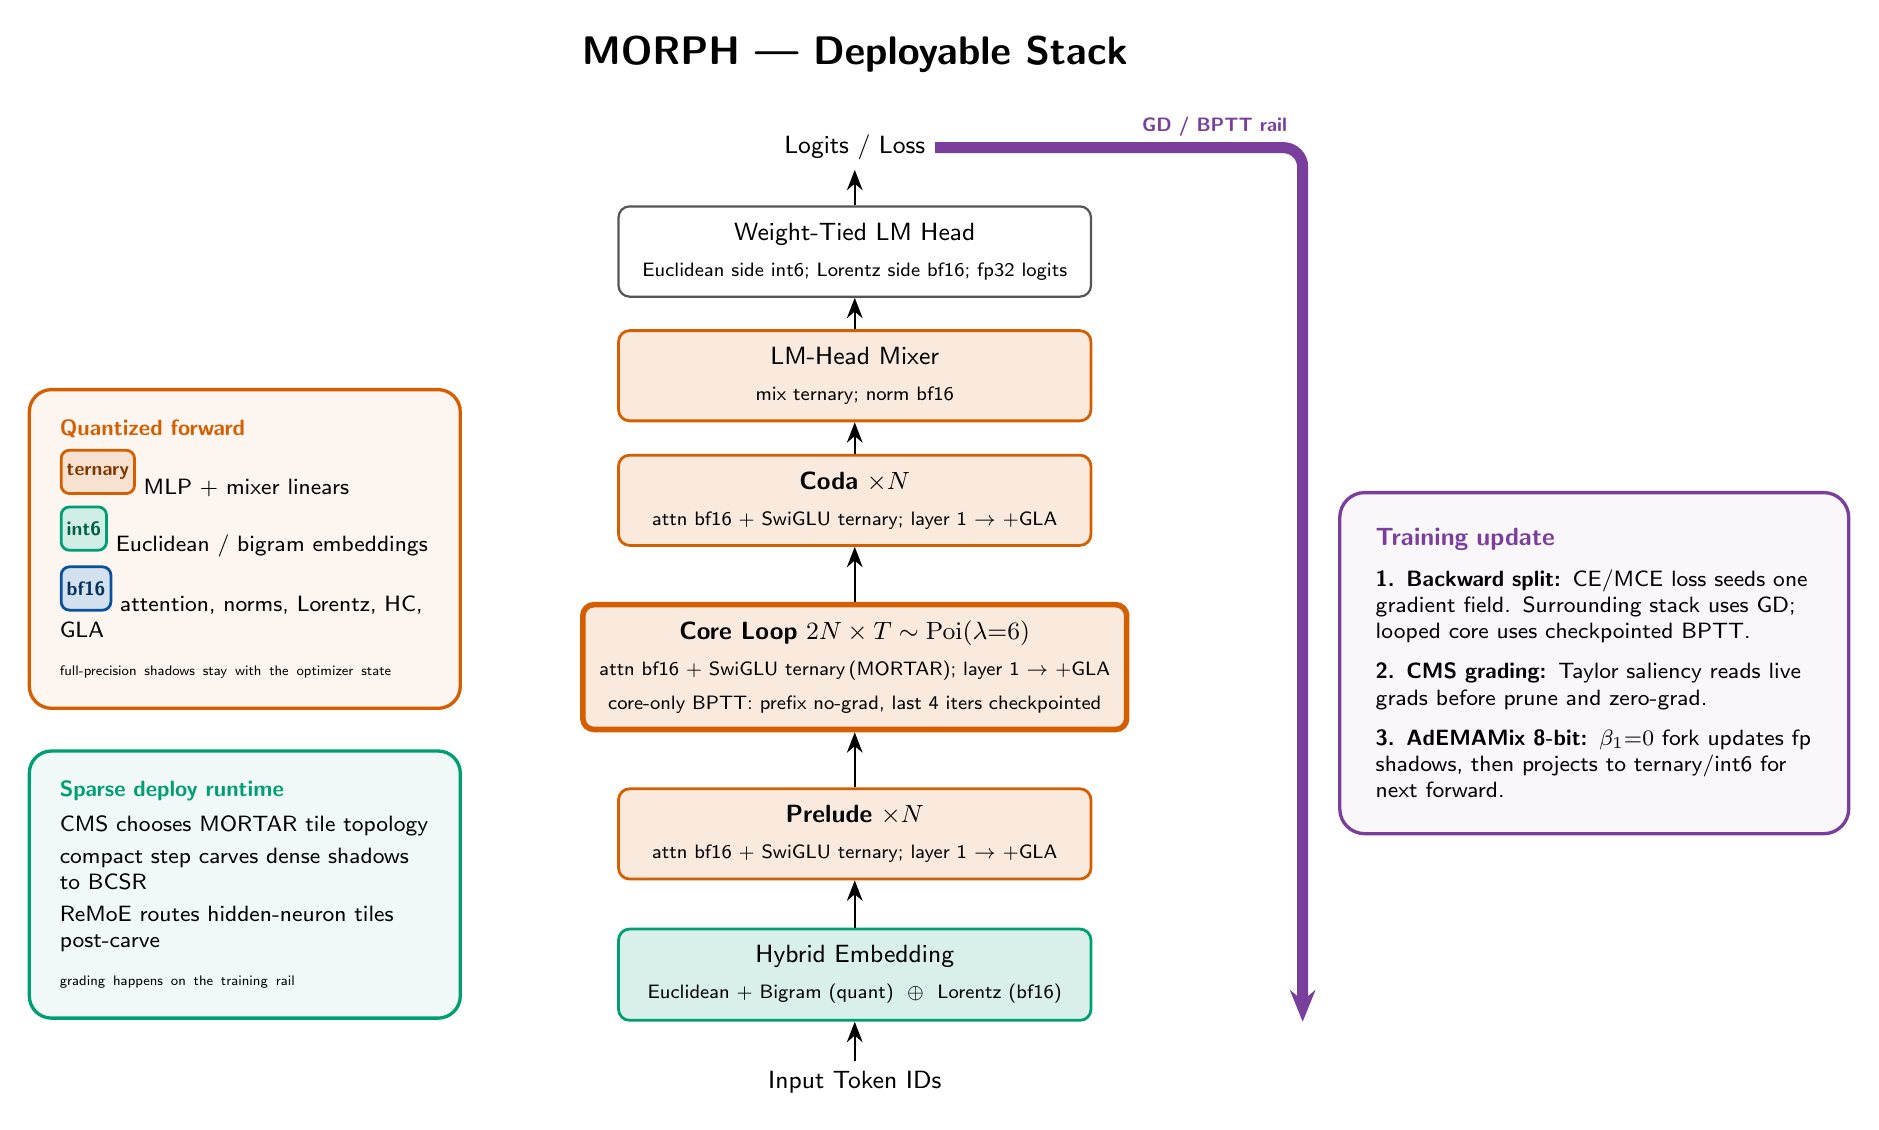
\begin{tikzpicture}[node distance=0.46cm]

% =====================================================================
% CENTRAL FORWARD-FLOW COLUMN  (input at bottom -> logits at top, matching overview)
% =====================================================================

\node[font=\small\sffamily] (inp) {Input Token IDs};

\node[PI6, above=0.5cm of inp] (emb) {
  Hybrid Embedding\\[2pt]
  {\scriptsize Euclidean + Bigram (quant) $\;\oplus\;$ Lorentz (bf16)}};
\draw[A] (inp) -- (emb);

\node[PT, above=0.6cm of emb] (pre) {
  \textbf{Prelude} $\times N$\\[2pt]
  {\scriptsize attn bf16 + SwiGLU ternary; layer 1 $\to$ +GLA}};
\draw[A] (emb) -- (pre);

% ── CORE LOOP (the heart) ────────────────────────────────────────────
\node[PT, above=0.7cm of pre, line width=2pt] (core) {
  \textbf{Core Loop} $2N \times T \sim \mathrm{Poi}(\lambda{=}6)$\\[2pt]
  {\scriptsize attn bf16 + SwiGLU ternary\,(MORTAR); layer 1 $\to$ +GLA}\\[1pt]
  {\scriptsize core-only BPTT: prefix no-grad, last 4 iters checkpointed}};
\draw[A] (pre) -- (core);

\node[PT, above=0.7cm of core] (coda) {
  \textbf{Coda} $\times N$\\[2pt]
  {\scriptsize attn bf16 + SwiGLU ternary; layer 1 $\to$ +GLA}};
\draw[A] (core) -- (coda);

\node[PT, above=0.4cm of coda] (mix) {
  LM-Head Mixer\\[2pt]{\scriptsize mix ternary; norm bf16}};
\draw[A] (coda) -- (mix);

\node[L, above=0.4cm of mix] (head) {
  Weight-Tied LM Head\\[2pt]
  {\scriptsize Euclidean side int6; Lorentz side bf16; fp32 logits}};
\draw[A] (mix) -- (head);

\node[font=\small\sffamily, above=0.45cm of head] (out) {Logits / Loss};
\draw[A] (head) -- (out);

% =====================================================================
% LEFT PANEL — deployment precision notes (no architecture formulas here)
% =====================================================================

\node[panel=pTern, anchor=east, text width=4.7cm] at ($(core.west)+(-1.50,1.5)$) (qscope) {
  \textbf{\textcolor{pTern}{Quantized forward}}\\[3pt]
  \tikz\node[badge=pTern, inner sep=2pt]{ternary};~MLP + mixer linears\\[2pt]
  \tikz\node[badge=pInt6, inner sep=2pt]{int6};~Euclidean / bigram embeddings\\[2pt]
  \tikz\node[badge=pBf16, inner sep=2pt]{bf16};~attention, norms, Lorentz, HC, GLA\\[4pt]
  {\tiny full-precision shadows stay with the optimizer state}};

\node[panel=pInt6, anchor=east, text width=4.7cm, below=0.5cm of qscope] (sparse) {
  \textbf{\textcolor{pInt6}{Sparse deploy runtime}}\\[3pt]
  CMS chooses MORTAR tile topology\\[2pt]
  compact step carves dense shadows to BCSR\\[2pt]
  ReMoE routes hidden-neuron tiles post-carve\\[4pt]
  {\tiny grading happens on the training rail}};

% =====================================================================
% RIGHT PANEL — GD/BPTT training rail
% =====================================================================

\node[draw=pTrain, very thick, rounded corners=9pt, fill=pTrain!4,
      text width=5.55cm, inner sep=13pt, align=left,
      font=\footnotesize\sffamily, anchor=west]
      (trainPanel) at ($(core.east)+(2.65,0.05)$) {%
  {\small\bfseries\textcolor{pTrain}{Training update}}\\[5pt]
  \textbf{1. Backward split:} CE/MCE loss seeds one gradient field. Surrounding stack uses GD; looped core uses checkpointed BPTT.\\[5pt]
  \textbf{2. CMS grading:} Taylor saliency reads live grads before prune and zero-grad.\\[5pt]
  \textbf{3. AdEMAMix 8-bit:} $\beta_1{=}0$ fork updates fp shadows, then projects to ternary/int6 for next forward.};

\coordinate (railTop) at ($(trainPanel.north west)+(-0.45,-0.60)$);
\coordinate (railBot) at ($(trainPanel.west |- emb.south)+(-0.45,0.00)$);
\draw[pTrain, line width=4.0pt, rounded corners=7pt,
      -{Stealth[length=4.0mm,width=3.2mm]}]
  (out.east) -- (railTop |- out.east) -- (railTop) -- (railBot);
\node[font=\scriptsize\sffamily\bfseries, text=pTrain, anchor=south east,
      fill=white, inner sep=2pt]
  at ($(railTop |- out.east)+(-0.12,0.06)$) {GD / BPTT rail};

% ── Title ────────────────────────────────────────────────────────────
\node[above=0.55cm of out, font=\Large\sffamily\bfseries]
  {MORPH --- Deployable Stack};

\end{tikzpicture}
\end{document}
